\subsection{Architectural Strategies}

The hardware is packaged on a black case of about 50cm to 20cm and 10cm hight. The case
for the hardware is light in weight and most of the livestock such as cattle and cow, sheep would not
feel the case weight. The decision I do not want to strain wight of the livestock that it end up
affect their growth

On the drawing board, I wanted a flexible solar pane to be used  as belt, that will
serve two purposes, Charge the battery inside the case and also hold the case in place
due to availability I only able to find a hard solar panel that can charge up to 6V.
This will affect the design, The final package, The case and all would look nice, but it will
be good enough to do a demonstration


\subsubsection{\textit{Tehchnologies used}}

The hardware, ESP32 Micro controller it is programmed using the C++ programming
language and the curl library was used to allow the ESP32 to communicate with
the server over the internet. C++ is the standard programming language when it
come to programming low level system, It can integrate very well with hardware.
Made sense to use C++ although is not the only language since we have
language such as C\# and Rust. C++ turned out to even have more advantage since
we also want to consume less power and it can be optimize to maximise the speed
of the CPU. Curl, is a open source library used in most C++ code base when need
to connect to the internet it is also light libra, it does not consume too much
power

The server, is developed with the JavaScript programming language using a
framework called Express. Running on a node server(the application). JavaScript
it has replaced PHP when you want to create a quick server. It has most security
feature and the is more resources online for libraries for absolute
anything you might want to do. The server is hosted on Linode, a cloud base
company that offer most cloud services. This is to make sure you can connect
to sever from anywhere around the world

Future plan for the application is to collect more data from the livestock such as temperature,
location and display the information in to the dashboard. Research on maximizing power efficient so that
the system can last longer on a single charge if the solar panel can not charge the battery in a
rainy weather.

The user interact with the system via a web browser. If they know how to user a web browser
They will know how to use the system. The input to the system is the signal sent from the case
to the server and the output will be the dashboard where we display the information about
the livestock


\subsubsection{\textit{Communication mechanisms used}}
\begin{figure}[htbp]
\centering
    \begin{subfigure}[b]{7cm}
        \centering
        % Primeira subfigura
        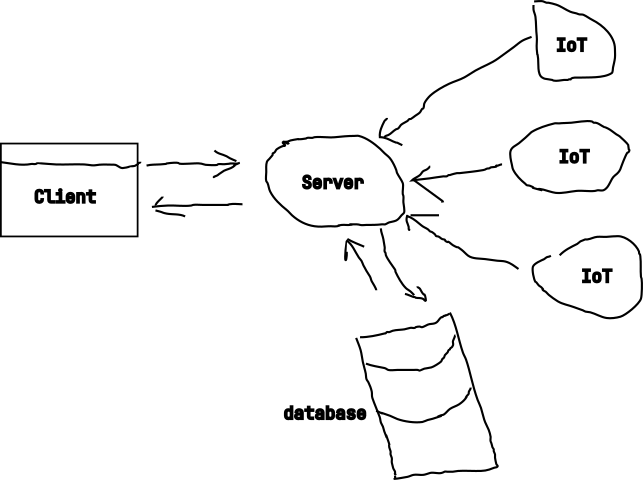
\includegraphics[width=7cm]{cc.png} % URI da subfigura
        \subcaption{
        % Legenda da subfigura
        data flow
        }
        \label{fig2:sub1}
    \end{subfigure}
\quad
    \begin{subfigure}[b]{7cm}
        \centering
        % Segunda subfigura
        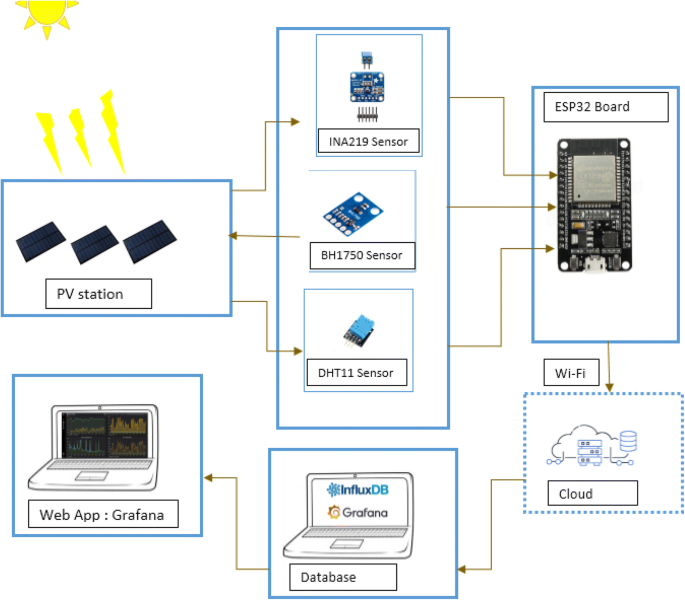
\includegraphics[width=7cm]{ccc.png} % URI da subfigura
        \subcaption{
        % Legenda da subfigura
        connection flow
        }
        \label{fig2:sub2}
    \end{subfigure}
\caption{
Communication diagram
}
\label{fig:fig2} % Tag para referência
\end{figure}

\subsection{Subsystem Architecture}

The system does not contain complicated componentes, everything is simple as it
archieve a specific things. This is by design, Thanks to the Unix philosophy. The
whole purpose of the system is to count livestock remotely


\subsubsection{\textit{ESP32(hardware)}}

For the system to be able to count livestock, E=each esp32 micro controller
get atatched to the livestock. The ESP32 the sends request to a remote server
with a uniquer UUID to identify the livestock. The request is being constantly send
to the server at an interval time rate

\subsubsection{\textit{Node Js (Server Application)}}

The Server application is connect to a Maria database and listening to HTTP request,
when a POST request is being made with UID, It gets save to the database with the time
stamp. The Server also expose a Web Socket to stream the total number of unique ID that are in the database.
When a client is connected to that socket, the total number its get send to the client

\subsubsection{\textit{Web Application (Client dashborad)}}
The Web applicaton connect to the server using web socket to listen to the datat bieng screaed from
the server which represent the number of unique ID from the databas

